\documentclass[a4paper,12pt]{article}
\usepackage{unifrsr}
\usepackage{float}
\usepackage{subcaption}
\usepackage{enumitem}
\usepackage{url}
\usepackage{hyperref}
\usepackage{pdfpages}
\usepackage[page,toc,titletoc,title]{appendix}
\usepackage{tocloft}
\usepackage{todonotes}
\usepackage[english]{babel}
\usepackage{csquotes}
\usepackage{pgfplots}
\pgfplotsset{compat=1.16}
\usepackage{enumerate}
\PassOptionsToPackage{%
backend=biber, % Instead of bibtex
% backend=bibtex8,
bibencoding=ascii,%
language=auto,%
style=numeric-comp,%
%style=authoryear-comp, % Author 1999, 2010
%bibstyle=authoryear,dashed=false, % dashed: substitute rep. author with ---
sorting=nyt, % name, year, title
maxbibnames=10, % default: 3, et al.
%backref=true,%
natbib=true % natbib compatibility mode (\citep and \citet still work)
}{biblatex}
\usepackage{biblatex}
\bibliography{references}
\usepackage{array,multirow,graphicx}


\usepackage{listings}

\begin{document}
\seminartitle{Social Media Analytics} % The title of the seminar

\title{Information Diffusion and Influence in Twitter } % The title of your project

\author{Hekuran Mulaki (16-217-382)\thanks{\email{hekuran.mulaki@unifr.ch}, University of Fribourg}
    \and Lionel Ieri (12-219-333)\thanks{\email{lionel.ieri@unifr.ch}, University of Fribourg}
   }	% Note: XX-XXX-XXX is the student's matriculation number
   % The author(s), separated by \and

\supervisor{Prof. Phillip, Mourad Kahaty} % Name of the supervisor

\assistant{Akansha \and Rana Hussein} %Name of the assistant(s)

\date{\today} % Note: if this is left out, today's date will be used, this is the submission date!

\maketitle

%should consist of about 150 words, describing the main results of our work



%\tableofcontents



\newpage



\DeclareFixedFont{\ttb}{T1}{txtt}{bx}{n}{12} % for bold
\DeclareFixedFont{\ttm}{T1}{txtt}{m}{n}{12}  % for normal

\definecolor{deepblue}{rgb}{0,0,0.5}
\definecolor{deepred}{rgb}{0.6,0,0}
\definecolor{deepgreen}{rgb}{0,0.5,0}
\definecolor{deeporange}{rgb}{.7,.5.0}
\lstdefinestyle{custompython}{
language=Python,
 basicstyle=\ttm,
 otherkeywords={self},             % Add keywords here
 keywordstyle=\ttb\color{deepblue},
 emph={MyClass,__init__},          % Custom highlighting
 emphstyle=\ttb\color{deepred},    % Custom highlighting style
 stringstyle=\color{deeporange},
 frame=tb,                         % Any extra options here
 showstringspaces=false,
 breaklines=true,
 numbers=left
 title=\lstname 
}

\section{Dataset}
The datasets consists of 3 different edgefiles, which represents different interactions of twitterusers. Since these are are one way interactions, the datasets each represents a directed graph.\\
 In order to recreate the informationflow, the graphs must be reversed and and summed up to represent one value per edge of an interaction. In the next step those new weights had to be normalized, and which was used as a base for our implementation and calculation.
\section{Implementation and Result Analysis}
In this chapter we will discuss the implementation of the ICM and greedy algorithm.
\subsection{Independent Cascade Model (ICM)}
The Independent cascade model is a stochastic information diffusion model where the information go through the network in a cascade. In such a model nodes can be either active or inactive. If a node is active it means that the node is already influenced by the information in the diffusion. On the other case, the node doesn't know anything about the information and is not influenced.
The information diffusion starts as follows: At the beginning some nodes receives the information. These nodes are known as seed nodes. This nodes are automatically active. In each step an active node can influence his inactive neighbor. If no activation happens then this node will never have again a chance to influence this exact neighbor. When a neighbor is activated depends on the probability on the edge between those 2 nodes, if the edgeweight is higher than the probability, then this neighbor will be activated, and can in the next step can activate his neighbor.

\subsection{Maximizing the spread of cascades - Greedy algorithm}

With a greedy algorithm our main focus was on optimising the cycle speed to facilitate the treatment of our dataset.
One of the first hurdle was to make the algorithm deterministic instead of stochastic for consistency. For that we're using the \href{https://docs.python.org/3.8/library/random.html#random.seed}{random.seed} from python random library, which will give us consistent generated values.

\begin{figure}[H]
    \centering
    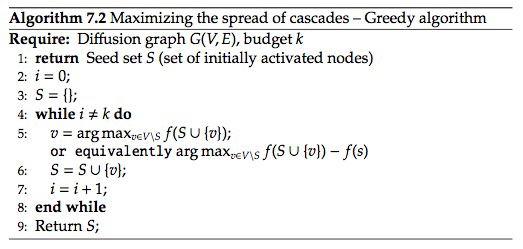
\includegraphics[width=0.8\linewidth]{Report/images/greedy_pseudo.png}
    \caption{Pseudocode of Greedy algorithm}
    \label{fig:greedy_pseudo}
\end{figure}

\noindent The first implementation was relatively inefficient. The cascades were calculated from scratch for each nodes each time we were trying to determine the highest spreading node (line 5 of the pseudocode in \ref{fig:greedy_pseudo}.)
To solve that we moved to calculate the activation for each nodes preemptively with \texttt{neighbors\_activation(G)} which check the potential for each node to activate its neighbours.
This accelerated the process, but was still slow. 

To optimise more, cascades were eventually move to be pregenerated to with \texttt{icm\_all(G, act)}. This gives us a dictionary of cascade for each nodes. With this the algorithm speed improve drastically.

\lstinputlisting[style=custompython, firstline=62, lastline = 83,firstnumber= 62]{../greedy.py}

\subsubsection*{Mistake and potential fix (Lionel)}

Unfortunately, on Friday I've spotted what I think is a mistake I've made with \texttt{pregen\_icm}, as line 38 calculate the longest cascade from one node instead of calculating the total number of activity.
For that, the lists of nodes from the cascade should be put together without repetition and counted. The different basic options I've tried to work with take an extremely long time which would not allow us to provide a result on time. This means that our results treating with the greedy ICM algorithm are flawed. We had already analysed them earlier, so our evaluation and discussion is based on the data we had available.

\section{Evaluation}
\subsection{ICM - Activation over time}
\begin{figure}[H]
    \centering
    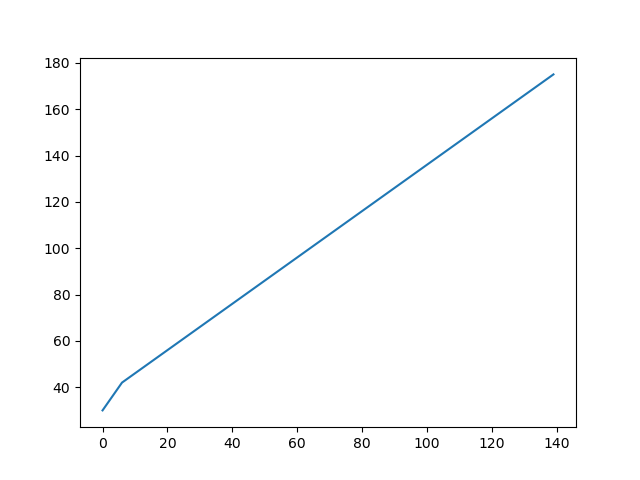
\includegraphics[width=0.5\linewidth]{Report/figs/ICM-0to1.png}
    \caption{Activation over iteration with p= 0 to 1}
    \label{fig:icm01}
\end{figure}
Since there was the error in the \texttt{pregen\_icm} function mentioned above, the pregenerated cascade was also used for this purpose, and so the results are not correct. If the results would be correct, we would expect an exponential rise of node activation, which would after some time flatten until no more activation happen.
\subsubsection{Lower the probability}
A quick glance at our data set shows that most nodes have only 1 interaction. Which lead to their value being normalized at 0. On the other hand, a handful of nodes have a lot of reach and have interacted and been interacted a lot. 
Which lead them to have a normalized value way way above the other values.
The consequences of that is that the mean value for our weight is low. 
Because of the low weights, an activation is not likely to happen. To be able to activate more nodes, we generate now a value between 0 and 0.1 and give them as a new probability.
\begin{figure}[H]
    \centering
    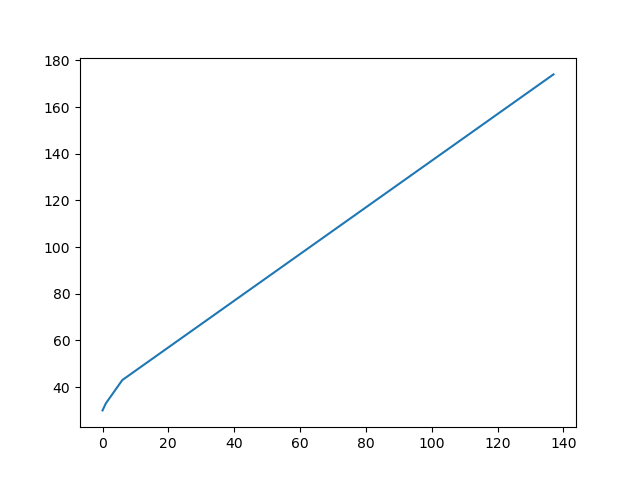
\includegraphics[width=0.5\linewidth]{Report/figs/ICM-0to01.png}
    \caption{Activation over iteration with p= 0 to 0.1}
    \label{fig:icm001}
\end{figure}
\noindent In such a case where you would lower the probabilities that much, there would be an big change of activation. But since the cascades are predefined, the activation will stay the same as with much higher probability values. In a normal situation, the curve should be exponentially until the end of the iteration, since almost every node could be activated.
\subsection{Greedy algorithm - variation of budget \textit{k}}
\begin{figure}[H]
\minipage{0.4\textwidth}
    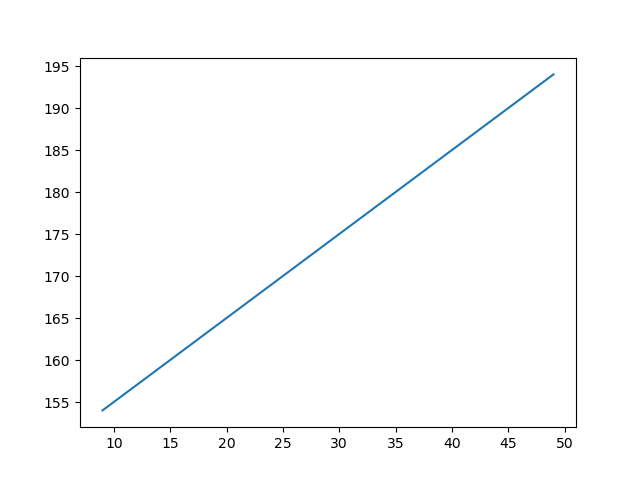
\includegraphics[width=\linewidth]{Report/figs/Greedy-0to1.png}
    \caption{Probabilities from 0 to 1}\label{fig:greedy01}
\endminipage\hfill
\minipage{0.4\textwidth}
    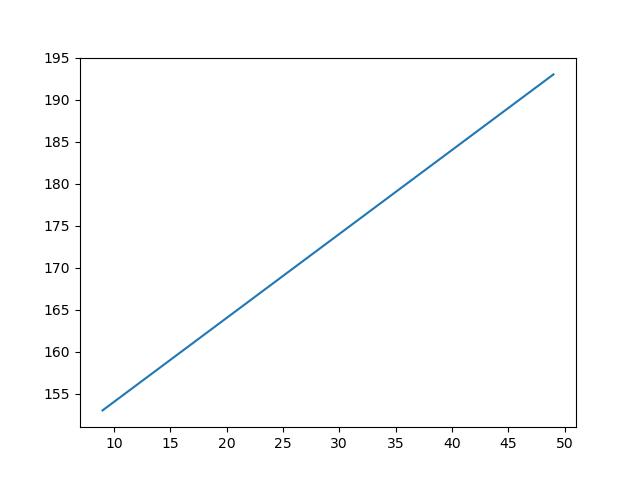
\includegraphics[width=\linewidth]{Report/figs/Greedy-0to01.png}
    \caption{Probabilities from 0 to 0.1}\label{fig:greedy001}
\endminipage
\end{figure}
By changing the budget k, the number of total activation should increase exponentially and after some time flatten, because we, but in our case we have a linear increase.
\subsection{Discussion of ICM}

The results of our Greedy ICM Algorithm are clearly problematic and it seems to clearly spark from the mistake in the implementation of the results. We spotted it once we started drawing the graph and by double checking the values. By verifying it, we also spotted that some nodes that should have a high cascade potentials are also missing from our list. Node 88, which has a lot of cascades starting from it is missing from our list of seeds, even with over 300 nodes.

\subsection{Pearson correlation}
To calculate the pearson coefficient we took each dataset individually and also the normalized graph.
To calculate the values we used the networkx library \textit{degree\_pearson\_correlation\_coefficient}, which gave us the following values:
\begin{center}
 \begin{tabular}{||c | c ||} 
 \hline
 Mention & -0.020746744677204432 \\
 \hline
 Reply & -0.04064928293680786\\ 
 \hline
 Retweet & 0.003181572224277474\\ 
 \hline
 Normalized & -0.020746744677204432 \\ 
 \hline
\end{tabular}
\end{center}
None of those nodes have a linear relation between them. The reason behind this could be the outliers in each of the dataset. Which received a value of 0 and only one connection
\subsection{Linear Threshold Model (LTM) over time}
The LTM is such a model where the weights of the edges between the nodes represent how much the nodes can affect each other. To be able to activate a neighbor, the sum of all incoming edges must be higher than the threshold, which was predefined. \\
For this part of the analyse we took 30 initial active nodes. Since the values of the nodes were really low, we did two different runs, once with pregenerating random value from 0 to 1, and once with values from 0 to 0.1. We came up with the following activation of nodes over iterations:
\begin{figure}[H]
\minipage{0.4\textwidth}
    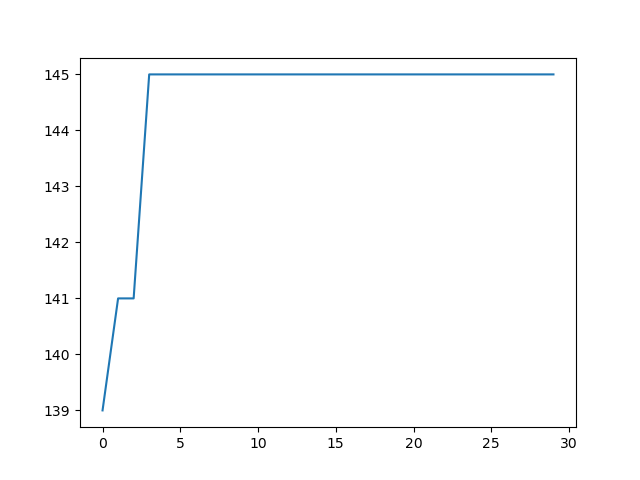
\includegraphics[width=\linewidth]{Report/figs/sumLTM-0to1.png}
    \caption{Probabilities from 0 to 1}\label{fig:sumLTM01}
\endminipage\hfill
\minipage{0.4\textwidth}
    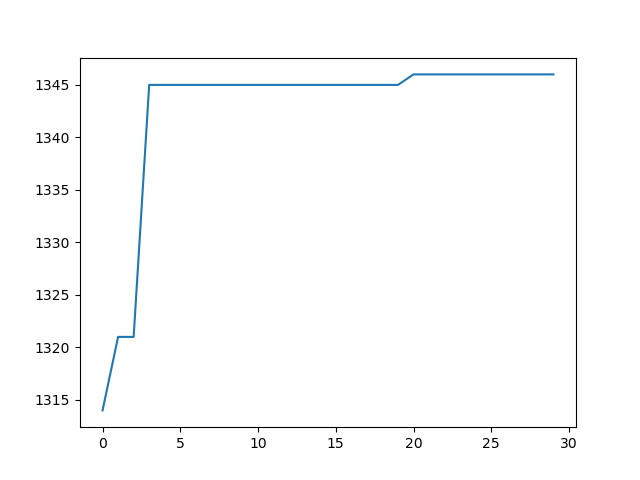
\includegraphics[width=\linewidth]{Report/figs/sumLTM.png}
    \caption{Probabilities from 0 to 0.1}\label{fig:sumltm}
\endminipage
\end{figure}
\newpage
\subsubsection{Analysis of LTM-results}
At first sight the graphs have similar behavior. What changes are the values on the y-axis. The iteration with the higher probability gives us less activation over 30 nodes, than then one with less higher probability. The reason behind this difference is that the normalized values are to low and by summing them up, they can't reach the threshold.\\

\subsection{General discussion}

The cascade model is definitely a powerful tool to analyse and target certain node in an analysis of a network similar to Twitter. While our implementation failed to show it, being able to isolate different nodes able to spread information to a wide network is crucial to understand the network if you aim to advertise in it or control it.
The nature of the greedy algorithm do lead to quite a deep complexity and while it may not be NP-Complete, it can still have a high complexity and cost.
Simply treating the spread of information through a deterministic with fixed values method allows an easier representation.
But the main issue will still be that in our implementation it deep rundown for each node each time, leading to a long time for analysis. 







\end{document}